% Chapter 3, Section 2: Conditional Probability and Bayes' Rule

\section{Conditional Probability and Bayes' Rule \difficultyInline{beginner}}
\label{sec:conditional-probability}

This section introduces the fundamental concepts of conditional probability and Bayes' theorem, which are essential for understanding how to update beliefs with new information in machine learning.

\subsection{Intuition: Updating Beliefs with New Information}

Imagine you're a doctor trying to diagnose a patient. Initially, you might think there's a 5\% chance the patient has a rare disease. But then the patient tells you they have a specific symptom that's present in 80\% of people with that disease. How should you update your belief?

This is exactly what \textbf{conditional probability} helps us do - it tells us how to update our beliefs when we get new information.

\subsection{Conditional Probability}

The conditional probability of $X$ given $Y$ is defined as:
\begin{equation}
P(X|Y) = \frac{P(X, Y)}{P(Y)}
\end{equation}
This quantifies how the probability of $X$ changes when we know the value of $Y$. This concept is fundamental to understanding how new information updates our beliefs about uncertain events, allowing us to make more informed decisions based on the evidence we observe.

\begin{examplebox}{Medical Diagnosis}
Let's make this concrete with our medical example:
\begin{itemize}
    \item $D$: Patient has the disease (1 = yes, 0 = no)
    \item $S$: Patient has the symptom (1 = yes, 0 = no)
\end{itemize}

From medical records, we know:
\begin{itemize}
    \item $P(D=1) = 0.05$ (5\% of population has the disease)
    \item $P(S=1|D=1) = 0.8$ (80\% of diseased patients have the symptom)
    \item $P(S=1|D=0) = 0.1$ (10\% of healthy patients have the symptom)
\end{itemize}

If a patient has the symptom, what's the probability they have the disease?

Using Bayes' theorem (which we'll derive next):
\begin{align}
P(D=1|S=1) &= \frac{P(S=1|D=1)P(D=1)}{P(S=1)} \\
&= \frac{0.8 \times 0.05}{0.8 \times 0.05 + 0.1 \times 0.95} \\
&= \frac{0.04}{0.04 + 0.095} \\
&= \frac{0.04}{0.135} \approx 0.296
\end{align}

So even with the symptom, there's only about a 30\% chance the patient has the disease!
\end{examplebox}

\subsection{Independence}

Two events are independent if knowing one doesn't change our belief about the other, such as rolling two dice where the result of the first die doesn't affect the second, or they can be dependent like weather and clothing choice where knowing it's raining affects the probability you'll wear a raincoat. Two random variables $X$ and $Y$ are independent if $P(X, Y) = P(X)P(Y)$, which means that the joint probability equals the product of the individual probabilities, or equivalently, $P(X|Y) = P(X)$ and $P(Y|X) = P(Y)$, indicating that knowing the value of one variable doesn't change our belief about the other.

\begin{examplebox}{Independent vs Dependent Variables}
Consider two scenarios:

\textbf{Scenario 1 (Independent):} Flipping two coins
\begin{itemize}
    \item $P(\text{First coin = Heads}) = 0.5$
    \item $P(\text{Second coin = Heads}) = 0.5$
    \item $P(\text{Both Heads}) = 0.5 \times 0.5 = 0.25$ \checkmark
\end{itemize}

\textbf{Scenario 2 (Dependent):} Drawing cards without replacement
\begin{itemize}
    \item $P(\text{First card = Ace}) = 4/52 = 1/13$
    \item $P(\text{Second card = Ace}) = 3/51$ (if first was Ace) or $4/51$ (if first wasn't Ace)
    \item The probability of the second card depends on what the first card was
\end{itemize}
\end{examplebox}

\subsection{Bayes' Theorem}

\subsubsection{Intuition: The Most Important Formula in Machine Learning}

Bayes' theorem is like a "belief update machine." It tells us how to revise our initial beliefs (prior) when we observe new evidence, to get our updated beliefs (posterior).

\begin{theorem}[Bayes' Theorem]
Bayes' theorem is fundamental to probabilistic inference:

\begin{equation}
P(X|Y) = \frac{P(Y|X)P(X)}{P(Y)}
\end{equation}
\end{theorem}

\subsubsection{Understanding Each Component}

In machine learning terminology:
\begin{itemize}
    \item $P(X)$ is the \textbf{prior} probability - what we believed before seeing the data
    \item $P(Y|X)$ is the \textbf{likelihood} - how likely the data is given our hypothesis
    \item $P(X|Y)$ is the \textbf{posterior} probability - what we believe after seeing the data
    \item $P(Y)$ is the \textbf{evidence} or marginal likelihood - the probability of observing the data
\end{itemize}

\subsubsection{Visualizing Bayes' Theorem}

\begin{figure}[h]
\centering
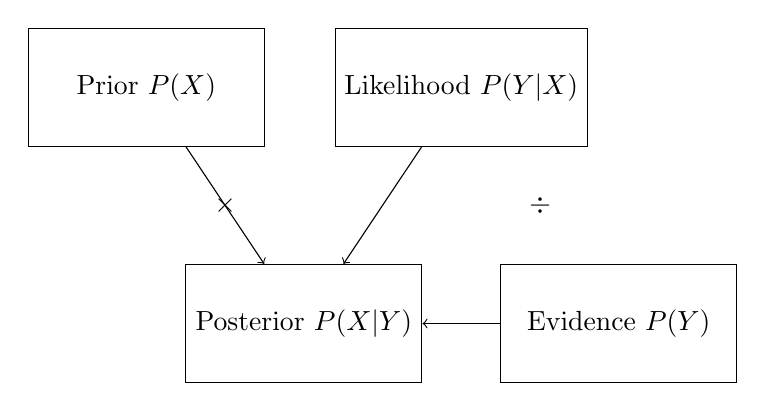
\begin{tikzpicture}
\node[draw, rectangle, minimum width=3cm, minimum height=1.5cm] (prior) at (0,0) {Prior $P(X)$};
\node[draw, rectangle, minimum width=3cm, minimum height=1.5cm] (likelihood) at (4,0) {Likelihood $P(Y|X)$};
\node[draw, rectangle, minimum width=3cm, minimum height=1.5cm] (posterior) at (2,-3) {Posterior $P(X|Y)$};
\node[draw, rectangle, minimum width=3cm, minimum height=1.5cm] (evidence) at (6,-3) {Evidence $P(Y)$};

\draw[->] (prior) -- (posterior);
\draw[->] (likelihood) -- (posterior);
\draw[->] (evidence) -- (posterior);

\node at (1,-1.5) {$\times$};
\node at (5,-1.5) {$\div$};
\end{tikzpicture}
\caption{Bayes' theorem as a belief update process}
\label{fig:bayes-process}
\end{figure}

The formula can be read as: "Posterior = (Likelihood × Prior) ÷ Evidence"

\subsection{Application to Machine Learning}

Bayes' theorem forms the basis of several important machine learning techniques. Bayesian inference provides a framework for updating beliefs about model parameters as new data becomes available, allowing for principled uncertainty quantification and decision-making under uncertainty. Naive Bayes classifiers use the assumption of feature independence to efficiently compute posterior probabilities for classification tasks, making them particularly useful for text classification and spam detection applications. Maximum a posteriori (MAP) estimation combines prior knowledge about parameters with observed data to find the most likely parameter values, providing a principled way to incorporate domain expertise into machine learning models. Bayesian neural networks extend traditional neural networks by treating weights as random variables with probability distributions, enabling uncertainty quantification in predictions and providing more robust estimates of model confidence.

Given data $\mathcal{D}$ and model parameters $\theta$:

\begin{equation}
P(\theta|\mathcal{D}) = \frac{P(\mathcal{D}|\theta)P(\theta)}{P(\mathcal{D})}
\end{equation}
